\documentclass[twocolumn]{el-author}

\usepackage{listings}

\lstset{language=,
basicstyle=\ttfamily\scriptsize,
frame=single,
breaklines=true}



\newcommand{\hH}{\hat{H}}
\newcommand{\D}{^\dagger}
\newcommand{\ua}{\uparrow}
\newcommand{\nc}{\newcommand}
\nc{\da}{\downarrow} \nc{\hc}{\hat{c}} \nc{\hS}{\hat{S}}
\nc{\bra}{\langle} \nc{\ket}{\rangle} \nc{\eq}{equation (\ref}
\nc{\h}{\hat} \nc{\hT}{\h{T}}\nc{\be}{\begin{eqnarray}}
\nc{\ee}{\end{eqnarray}}\nc{\rd}{\textrm{d}}\nc{\e}{eqnarray}\nc{\hR}{\hat{R}}\nc{\Tr}{\mathrm{Tr}}
\nc{\tS}{\tilde{S}}\nc{\tr}{\mathrm{tr}}\nc{\8}{\infty}\nc{\lgs}{\bra\ua,\phi|}\nc{\rgs}{|\ua,\phi\ket}
\nc{\hU}{\hat{U}}\nc{\lfs}{\bra\phi|}\nc{\rfs}{|\phi\ket}\nc{\hZ}{\hat{Z}}\nc{\hd}{\hat{d}}\nc{\mD}{\mathcal{D}}
\nc{\bd}{\bar{d}}\nc{\bc}{\bar{c}}\nc{\mc}{\mathcal}\nc{\ea}{eqnarray}\nc{\mG}{\mathcal{G}}\nc{\bce}{\begin{center}}
\newcommand{\BB}[2]{\rule{0pt}{#1}\rule[#2]{0pt}{0pt}}
\nc{\ece}{\end{center}}
\date{12th April 2013}

\begin{document}

\title{Digital assistance for energy reduction in ADCs using a signal prediction algorithm}

\author{D. Avila, E. Alvarez and A. Abusleme}

\abstract{With the adoption of new technologies for analogue circuits, different digital techniques have been designed to enhance their performance. Among the existing techniques, a promising approach is to adapt the circuit operation dynamically considering the application characteristics. In the field of analogue-to-digital converters (ADCs), typically this approach is carried out by taking advantage of \mbox{application-dependent} signal properties, hence their use is limited. In this work, a digital assistance technique for power reduction in ADCs is presented. By defining a range for the next sample based upon the maximum possible change of the input signal between samples, the proposed algorithm reduces the mean energy consumption per conversion in a variety of ADC architectures, regardless of the application.}

\maketitle

\section{Introduction}

Digital assistance is used to expand the performance envelope of analogue circuits by taking advantage of the fast growing performance of digital circuits resulting from the technology scaling \cite{1}. Among the existing digital assistance techniques, a promising approach is to adapt the circuit operation dynamically according to the characteristics of its input signal, for example, in order to reduce the overall energy consumption. Several applications using this approach can be found in the design of ADCs for \mbox{high-efficiency}, \mbox{low-power} applications \cite{3,4,5,6}. Typically, this approach is carried out by using \mbox{application-dependent} signal characteristics, such as periodical changes in the input signal rate or the input signal expected shape. For this reason, these techniques lack generality and can only be used in specific applications. In this work, a digital assistance technique for energy reduction in \mbox{general-purpose} ADCs is presented. 

When designing an ADC for a custom IC, the maximum rate of change of the ADC input signal can be determined from the frequency bandwidth of the stage preceding to the ADC, typically a \mbox{signal-conditioning} stage. Using this parameter and the ADC sampling frequency, an expression for the maximum variation between samples of the ADC output can be computed. If the maximum possible change of the input signal between samples is limited, some of the most significant bits (MSBs) of the ADC output will remain constant between two consecutive samples, and for the next conversion, a part of the resulting bits are known already. Skipping the MSBs that remain constant, the ADC only needs to compute the bits that are subject to change, thus reducing the mean energy consumption per conversion. For instance, in flash ADCs, for each MSB that remains constant this technique allows to turn off half of the comparators, whereas in \mbox{bit-at-a-time} ADCs, this technique allows a higher sampling rate when operating asynchronously, resulting in an energy saving proportional to the mean number of bits that remain constant between two conversions.

\section{Maximum variation of the ADC output}
The maximum variation between consecutive samples of the ADC input voltage, $\Delta v_\mathit{in,max}$, can be calculated considering that $v_\mathit{in}$ is maintained at its maximum rate of change for a complete sampling period, as illustrated in Fig.~\ref{fig:maxVar}. Mathematically, $\Delta v_\mathit{in,max}$ can be written as
\begin{equation}
 \Delta v_\mathit{in,max}   = \left|\frac{\mathrm{d}v_\mathit{in}}{\mathrm{d}t}(t)\right|_\mathit{max} \times \frac{1}{f_s} \label{eq:maxVar}
\end{equation}
where $\textstyle \left|\mathrm{d}v_\mathit{in}/\mathrm{d}t\;(t)\right|_\mathit{max}$ is the maximum rate of change of $v_\mathit{in}$ and $f_s$ is the ADC sampling frequency. The maximum variation of the ADC output between consecutive samples, $N$, can be written as a function of $\Delta v_\mathit{in,max}$  as follows
\begin{equation}
N = \left\lceil \frac{\Delta v_\mathit{in,max}}{\mathit{LSB}} \right\rceil \label{eq:N1}
\end{equation}
where $\mathit{LSB} = \mathit{FSR}/ 2^B$ is the code length, $\mathit{FSR}$ is the ADC full scale range, $B$ is the ADC stated resolution in bits, and $\left\lceil\cdot\right\rceil$ is the ceiling function.
\begin{figure}[!h]
	\centering
	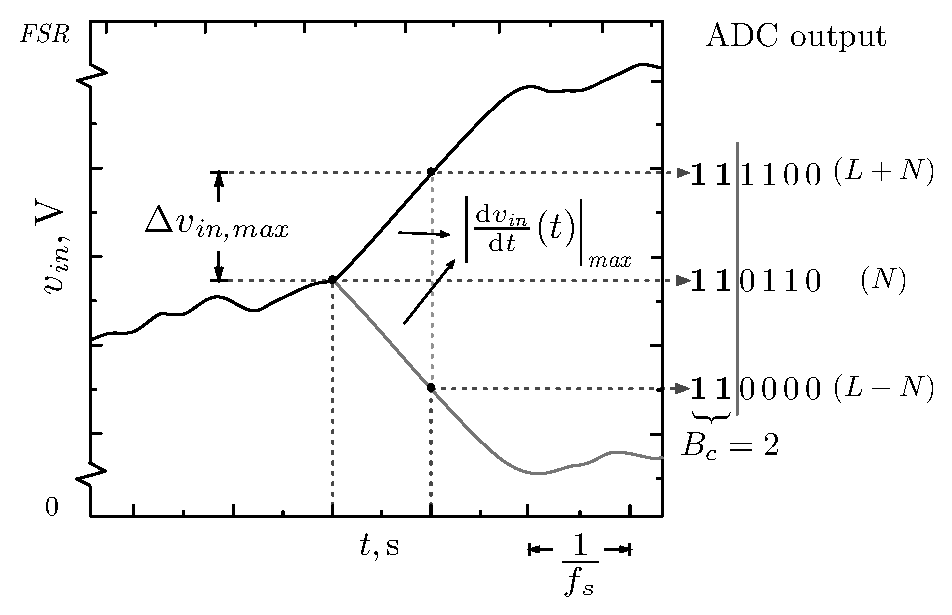
\includegraphics[width=3.3in]{graph.eps}
	\caption{Illustration of the maximum voltage variation at the ADC input.}
	\label{fig:maxVar}
\end{figure}

For illustration purposes, let us suppose that the bandwidth of $v_{in}$ is limited by a brick-wall filter with a \mbox{cut-off} frequency of \mbox{$f=\mathit{BW}$}. Considering this, the maximum rate of change of $v_{in}$ is given by the maximum slope of a sine wave of frequency $BW$ and peak amplitude $\mathit{FSR}/2$. Therefore, \eqref{eq:N1} can be written as a function of the ADC input voltage bandwidth as
\begin{equation}
N = \left\lceil \frac{\pi \times \mathit{BW} \times \mathit{FSR}}{\mathit{LSB}} \times \frac{1}{f_s}\right\rceil  = \left\lceil \frac{2^{B-1}\times\pi}{\mathit{OSR}}\right\rceil \label{eq:Nfinal}
\end{equation}
where $\mathit{OSR}=f_s/\left(2\times\mathit{BW}\right)$ is the oversampling ratio. In a practical design, $N$ must be calculated considering the actual frequency response of the stage prior to the ADC.

\section{Algorithm}
Considering that the maximum variation of the ADC output between two consecutive samples is $\pm N$, the proposed algorithm works as follows: once the current digital output $L$ is computed, a variation of $\pm N$ is applied to $L$ and the results given by \mbox{$\text{min}(L+N, 2^B-1)$} and \mbox{$\text{max}(L-N,0)$} are bitwise compared to $L$ in order to determine $B_c$, which is the number of MSBs that will remain constant in the following conversion. Fig.~\ref{fig:algorithm} shows a pseudo code implementation for the proposed algorithm, which has been formulated to be written in a hardware description language to synthesize a combinational digital circuit.
\begin{figure}[!h]
\centering
\begin{lstlisting}[mathescape]
 a = max(L-N,0) $\oplus$ L
 b = min(L+N,2^B-1) t L
 c = a $\oplus$ b
 Bc = clz(c)
\end{lstlisting}
\caption{Pseudo code for the proposed algorithm. The operand $\oplus$ is the bitwise exclusive OR operator and clz is the count leading zeroes function.}\label{fig:algorithm}
\end{figure}

Using this algorithm, the operation of an ADC can be adapted considering that the $\mathit{B}_c$ MSBs of the following conversion are already known, so there is no need to compute them again and the mean energy consumption per conversion can be reduced.

In order to compute the mean number of bits that remain constant between two consecutive conversions, $\overline{\mathit{B}_c}$, an expression for the number of codes whose $i$ MSBs remain constant after a variation of $\pm N$ LSBs, $C_i$, should be computed first as follows
\begin{equation}
C_i = \hspace*{-0.1em}
\begin{cases}
2(2^x-N) & i = B-x \\
 2(2^{B-i}\hspace*{-0.3em}-\hspace*{-0.1em}N)\hspace*{-0.1em}+\hspace*{-0.1em}(2^i\hspace*{-0.1em}-\hspace*{-0.1em}2)(2^{B-i}\hspace*{-0.3em}-\hspace*{-0.1em}2N)-\hspace*{-0.8em}  \sum\limits_{j=i+1}^{B-x} \hspace*{-0.5em}C_j & i=2\ldots B\hspace*{-0.1em}-\hspace*{-0.1em}x\hspace*{-0.1em}-\hspace*{-0.1em}1 \vspace*{-4pt}\\
 2^B-2N - \sum\limits_{j=2}^{B-x} C_j  & i=1 \\
\end{cases}\label{eq:Bi}
\end{equation}
where $x = \left\lceil \log_2(N+1)\right\rceil$.

Assuming an uniformly distributed input, $\overline{\mathit{B}_c}$ can be calculated as 
\begin{equation}
\overline{\mathit{B}_c} = \frac{1}{2^B}\sum_{i=1}^{B-x} i \times C_i \label{eq:SB}
\end{equation}

Replacing \eqref{eq:Bi} in \eqref{eq:SB}, it can be seen that $\overline{\mathit{B}_c}$ only depends on the $\mathit{OSR}$, and not on the stated resolution of the ADC.

A variation of the proposed algorithm can be formulated for asynchronous \mbox{bit-at-a-time} ADCs. In these ADCs, the conversion time depends on $\mathit{B}_c$. Therefore, $N$ is not constant and can be recalculated at the end of each conversion. Assuming that the reset of the ADC takes one clock period, at the $i$-th conversion, $N_i$ can be computed dynamically as
\begin{equation}
N_i = \left\lceil \frac{2^{B-1}\times \pi}{\mathit{OSR}} \times \frac{B-\mathit{B}_{c,i-1}+1}{B+1}\right\rceil. \label{eq:Nfinal}
\end{equation} 

It can be seen that under this variation, the number of bits that remain constant between two consecutive conversions depends on the signal shape and not on the signal statistics, thus, $\overline{\mathit{B}_c}$ cannot be calculated for asynchronous operation.

\section{Behavioural simulation results}
The proposed algorithm and its variation with dynamic calculation of $N$ for asynchronous operation were simulated for a \mbox{$10$-bit} ADC. Both algorithms were tested using an input ramp spanning the full scale range, and using an input sine wave with a peak amplitude of $\mathit{FSR/2}$ and frequency $f=\mathit{BW}$. 

Table \ref{table:results} shows $\overline{\mathit{B}_c}$ for different values of $\mathit{OSR}$. As mentioned earlier, $\overline{\mathit{B}_c}$ does not depend on $B$, so the results shown in Table \ref{table:results} are also valid for a generic $B$-bit converter. Using these results and considering the ADC architecture, the mean saved energy consumption per conversion can be estimated. For instance, in a Flash ADC each bit that remains constant between two consecutive conversions allows to turn off  $50\,\%$ of the comparators, thus, a mean energy reduction of $18.37\,\%$ can be reached for $\mathit{OSR}=4$, whereas a mean energy reduction of $45.32\,\%$ can be reached for $\mathit{OSR}=8$. 
\begin{table}[!h]
\centering
\begin{tabular}{|l|c|c|c|c|}\hline
 $\mathit{OSR}$ & 2 & 4 & 8 & 16 \\\hline 
$\mathit{FSR}$ ramp, static $N$ & 0 & 0.21 & 0.71 &  1.27 \\ 
$\mathit{FSR}$ ramp, dynamic $N$ & 0 &  0.27 & 0.85 & 1.50 \\ 
$\mathit{FSR}\sin(2 \times \pi \times \mathit{BW})/2$, static $N$ & 0 & 0.73 & 1.59 & 2.42 \\ 
$\mathit{FSR}\sin(2 \times \pi \times \mathit{BW})/2$, dynamic $N$ & 0 &  0.77 & 1.67 & 2.56 \\\hline  
\end{tabular}
\vspace{0.1cm}
\caption{Simulated $\overline{\mathit{B}_c}$ as a function of $\mathit{OSR}$.}
\label{table:results}
\end{table}


\section{Conclusion}
A technique to reduce the mean number of bits processed per conversion is presented. The technique is based on estimating a range for the next ADC output and adapt the operation of the circuit accordingly.
The implementation of the technique is based on an algorithm that can be synthesized in a simple combinational digital circuit.
Additionally, the algorithm allows an speed improvement in asynchronous \mbox{bit-at-a-time} ADCs.

\vskip3pt
\ack{The authors thank the National Comission for Scientific and Technological Research (CONICYT) of Chile, through project FONDECYT 11110165, for the funding provided for this research.}

\vskip5pt

\noindent D. Avila, E. Alvarez and A. Abusleme (\textit{Department of Electrical Engineering Pontificia Universidad Cat\'olica de Chile, PO Box 306 - Correo 22, Santiago 7820436, Chile})
\vskip3pt

\noindent E-mail: dlavila@uc.cl

\begin{thebibliography}{}

\bibitem{1}
Murmann, B.: `Digitally Assisted Analog Circuits', \textit{Micro. IEEE} , 2006, \textbf{26}, no.2, pp. 38-47.

\bibitem{3}
Trakimas, M.; Sonkusale, S.R., `An Adaptive Resolution Asynchronous ADC Architecture for Data Compression in Energy Constrained Sensing Applications', \textit{Tran. on Circ. and Sys I}, 2011, \textbf{58}, no.5, pp. 921-934.

\bibitem{4}
O'Driscoll, S.; Shenoy, K.V.; Meng, T.H., `Adaptive Resolution ADC Array for an Implantable Neural Sensor', \textit{IEEE Trans. on Biom. Cir. and Sys.} , 2005, \textbf{5}, no.2, pp. 120-130.

\bibitem{5}
Zaare, M.; Sepehrian, H.;  Maymandi-Nejad, M.; `A New Non-Uniform Adaptive-Sampling Successive Approximation ADC for Biomedical Sparse Signals', \textit{Analog Integrated Circuits and Signal Processing}, 2013, \textbf{74}, no.2, pp. 317-330.

\bibitem{6}
Harpe, P.; Cantatore, E.; van Roermund, A., `A 2.2/2.7fJ/conversion-step 10/12b 40kS/s SAR ADC with Data-Driven Noise Reduction', \textit{Tech. Dig. IEEE Int. Solid-State Circ. Conf.} , 2013, pp. 270-271.


\end{thebibliography}

\end{document}
